\documentclass{beamer}
\usepackage[style=alphabetic]{biblatex}
\addbibresource{bibliography.bib}

\usetheme{CambridgeUS}
\logo{
\includegraphics[width=1.3cm]{images/logo}}

\title[Hate speech at meta]{Hate speech at meta\\ \footnotesize{How
    contrasting hate speech online is a core part of Meta social
    business model}}

\author{Luca Zaninotto}
\institute{Univerità di Padova}
\date{\today}

\begin{document}

\begin{frame}
  \titlepage
\end{frame}

\begin{frame}{Overview}
  \tableofcontents
\end{frame}

\section{Introduction -- Meta as a company}
\begin{frame}
  \begin{center}
    
\includegraphics[width=.5\textwidth]{images/meta_logo}
    \vfill
    \begin{itemize}
    \item in 2004, Mark Zuckerberg founds TheFacebook, an innovative
      and groundbraking social media
    \item Constantly growing since then
    \end{itemize}
    \vfill
  \end{center}
\end{frame}

\begin{frame}{Monthly active users worldwide}
  \begin{figure}
    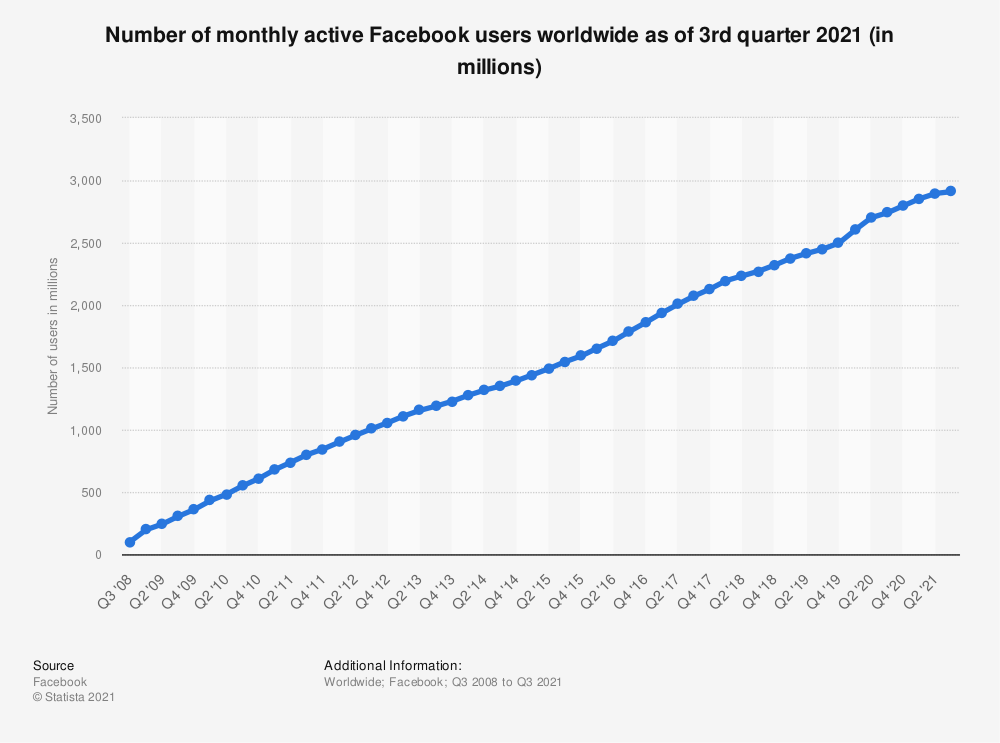
\includegraphics[width=.8\textwidth]{images/statista_MAU.png}
  \end{figure}
\end{frame}

\begin{frame}{Revenues}
  \begin{figure}
    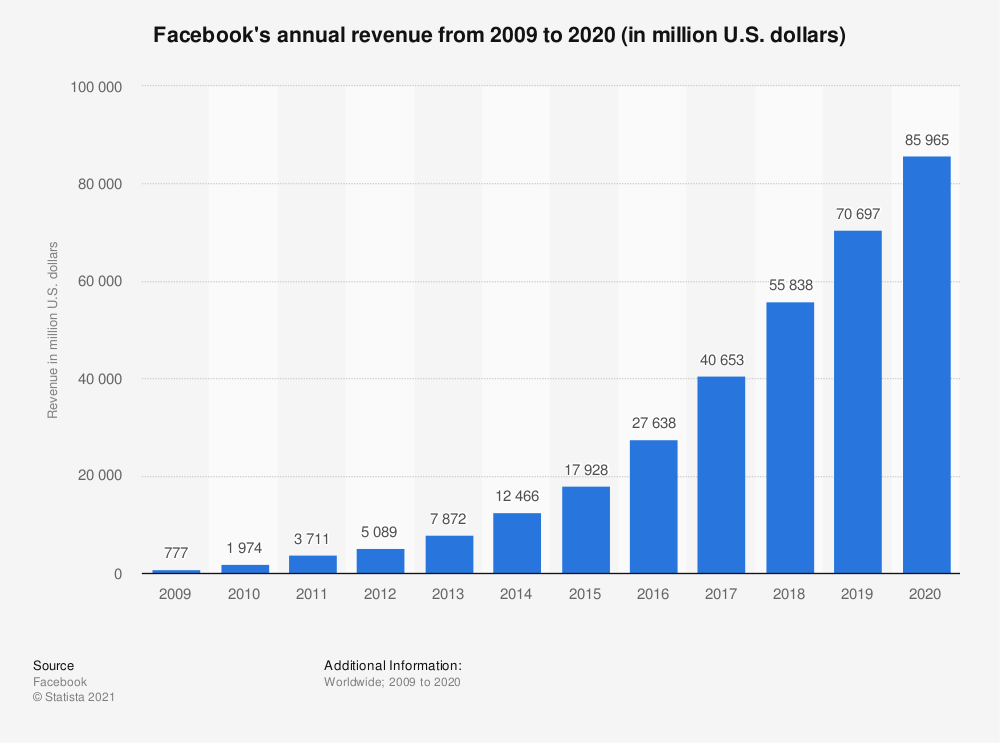
\includegraphics[width=.8\textwidth]{images/statista_rev.png}
  \end{figure}
\end{frame}

\begin{frame}{The other part of the story}
  \begin{itemize}
  \item In 2012 Facebook buys Instagram for 1 Billion dollars
  \item In 2014 Facebook buys WhatsApp for 19 Billion dollars
  \item In 2021 the company changes its brand to Meta
    platforms. Along with that they communicated that the new main
    goal of the firm was to build the ``metaverse''.
  \end{itemize}
\end{frame}

\section{Meta business model}
\begin{frame}{Core applications}
  \begin{figure}
    
\includegraphics[width=.4\textwidth]{images/fb.png}
    \hfill
    
\includegraphics[width=.4\textwidth]{images/ig.png}
  \end{figure}
\end{frame}

\begin{frame}{Meta social platforms business model}
  \begin{figure}
    \centering
    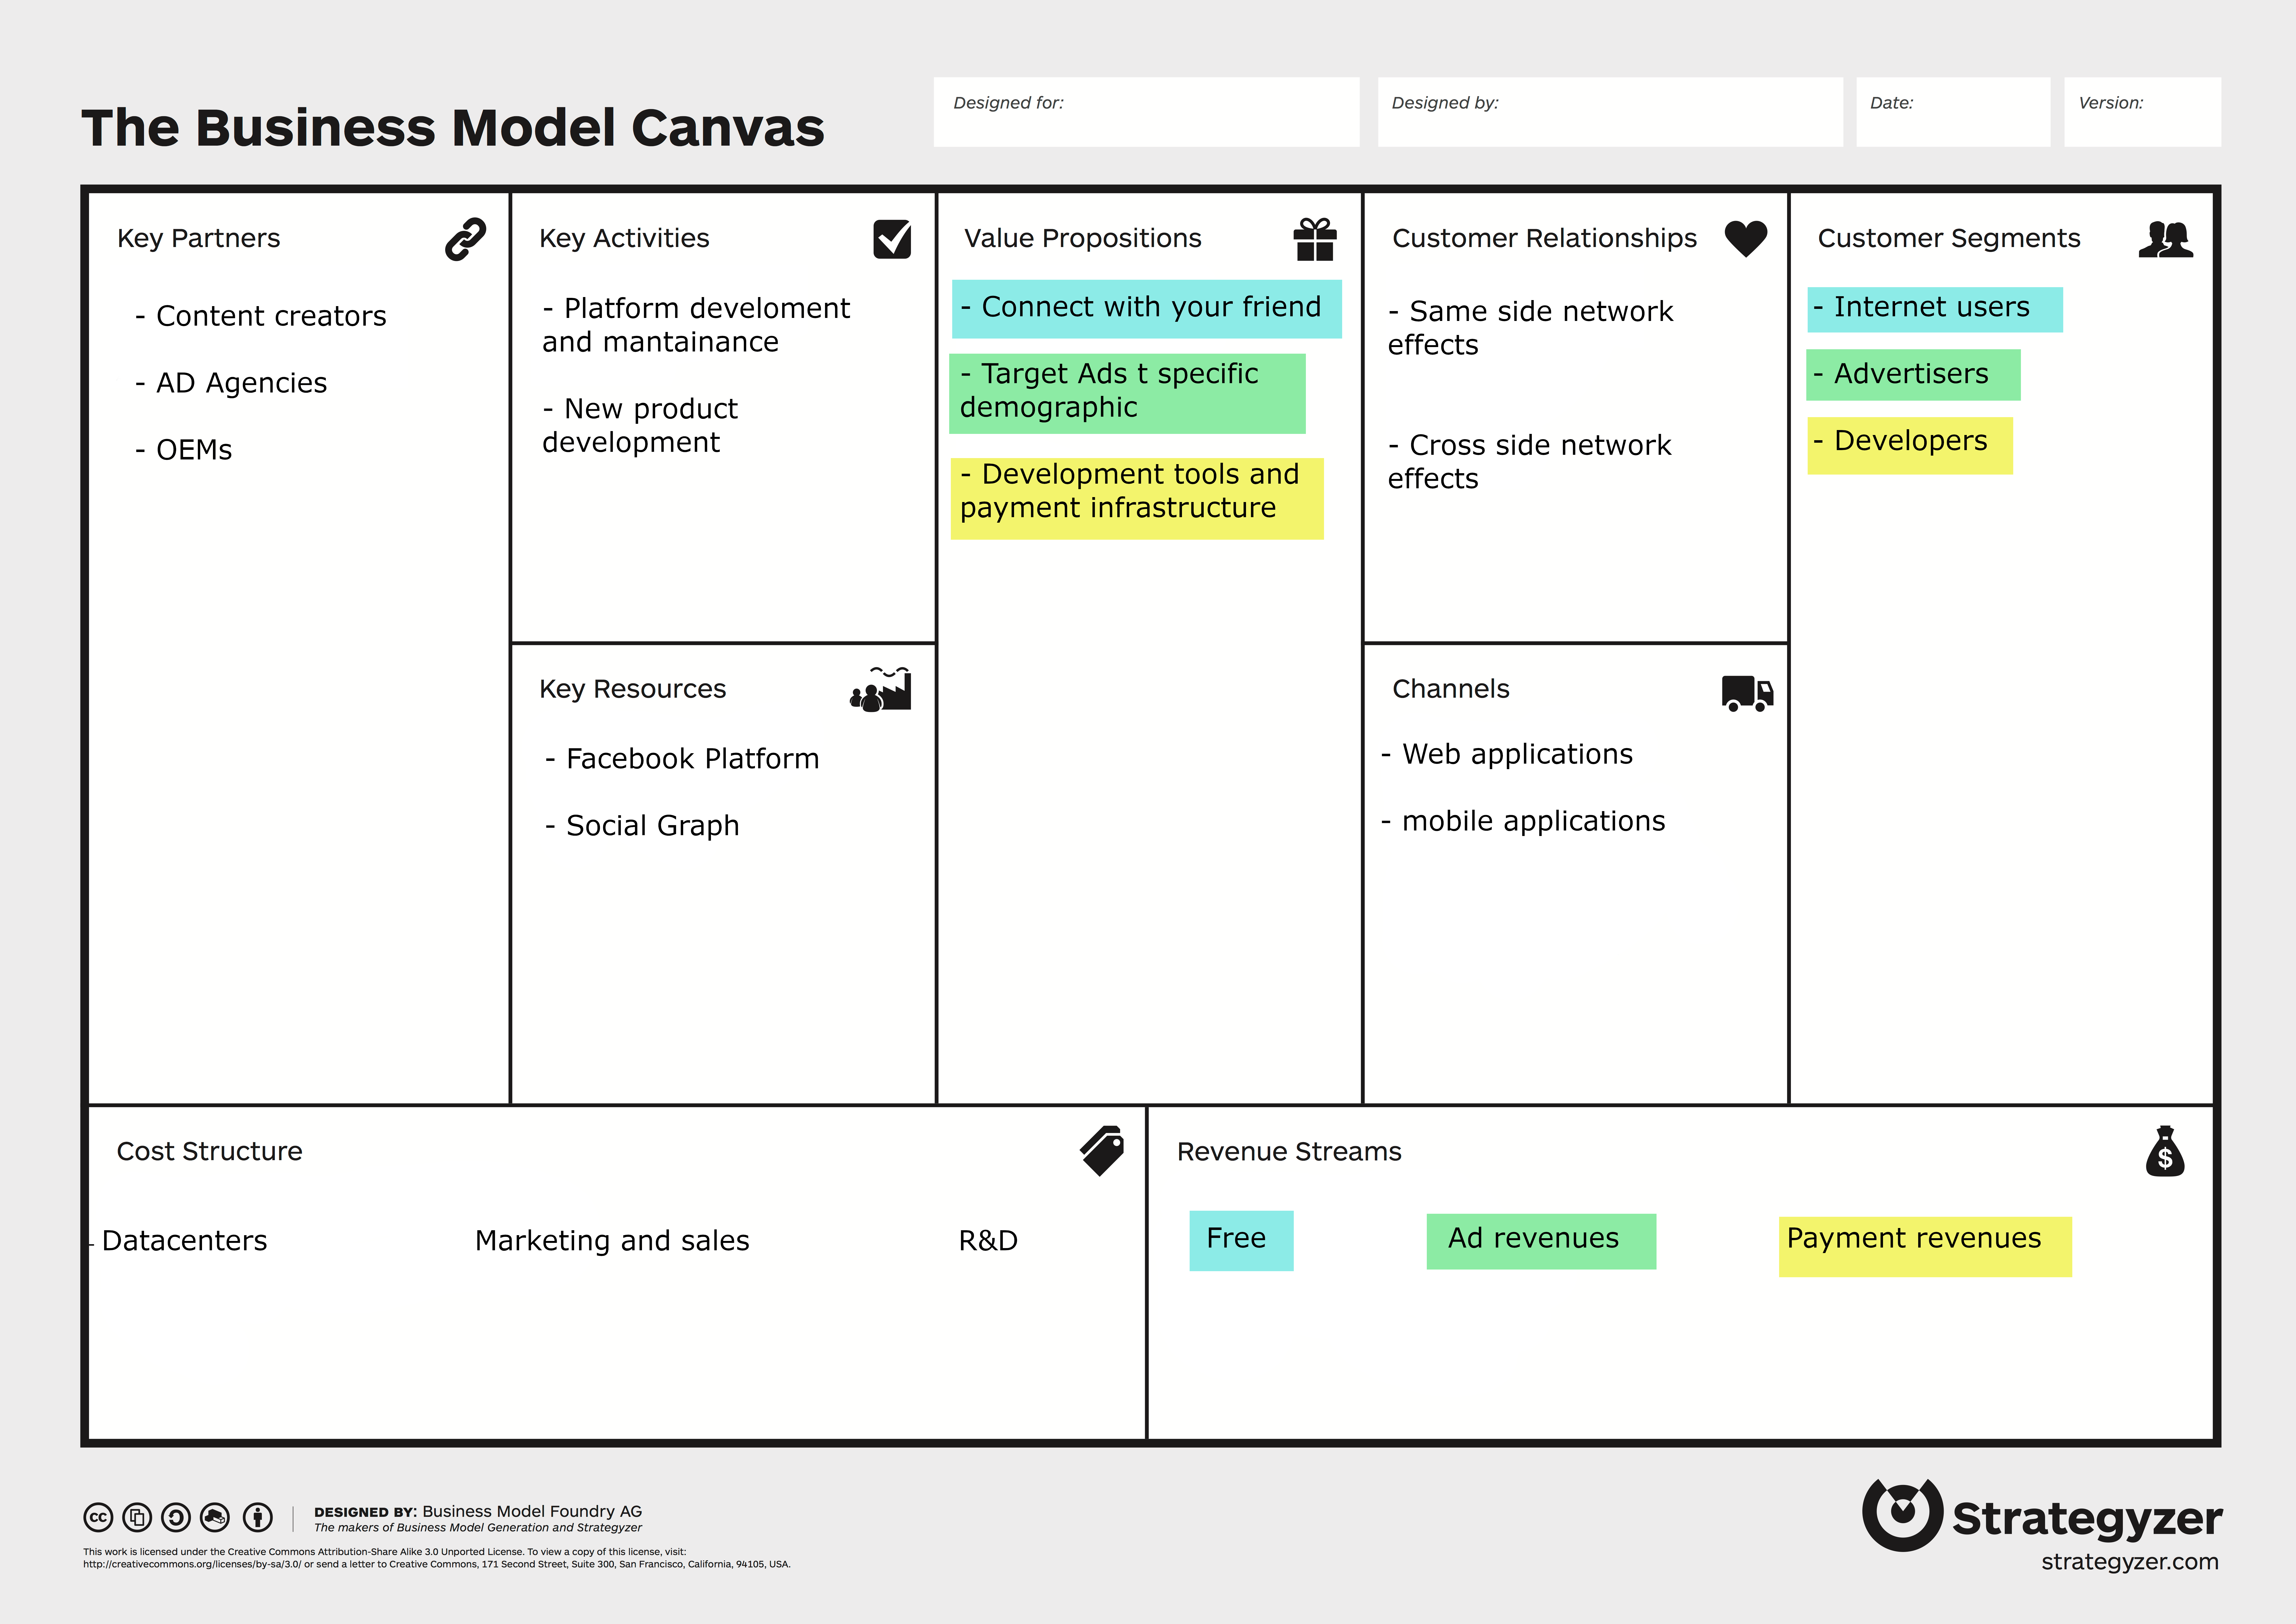
\includegraphics[width=\textwidth]{images/fbcanvas}
  \end{figure}
\end{frame}

\begin{frame}{Key factors}
  \begin{itemize}
  \item The relationship with customers is a key component of Meta
    business model.
  \item Factors that create a sense of distrust between the company
    and the customers puts in real danger the whole system.
  \end{itemize}
\end{frame}

\begin{frame}{Hate speech}
  \begin{itemize}
  \item Huge amount of users leads to different subgroups, one in
    contrast with the other.
  \item Misleading content that promotes violence
  \item Users dont want to see harmful content
  \item Advertisers dont want their products associated to harmful
    content
  \end{itemize}
\end{frame}

\section{Innovative AI}
\begin{frame}{A continuous journey}
  \begin{itemize}
  \item Meta started in 2016 to use AI to detect harmful content
    online
  \item New and new technologies started to emerge in order to
    contrast HS since then.
  \item One of the main problems was the evolution of language
  \end{itemize}
\end{frame}

\begin{frame}{New model}
  \begin{figure}
    \centering
    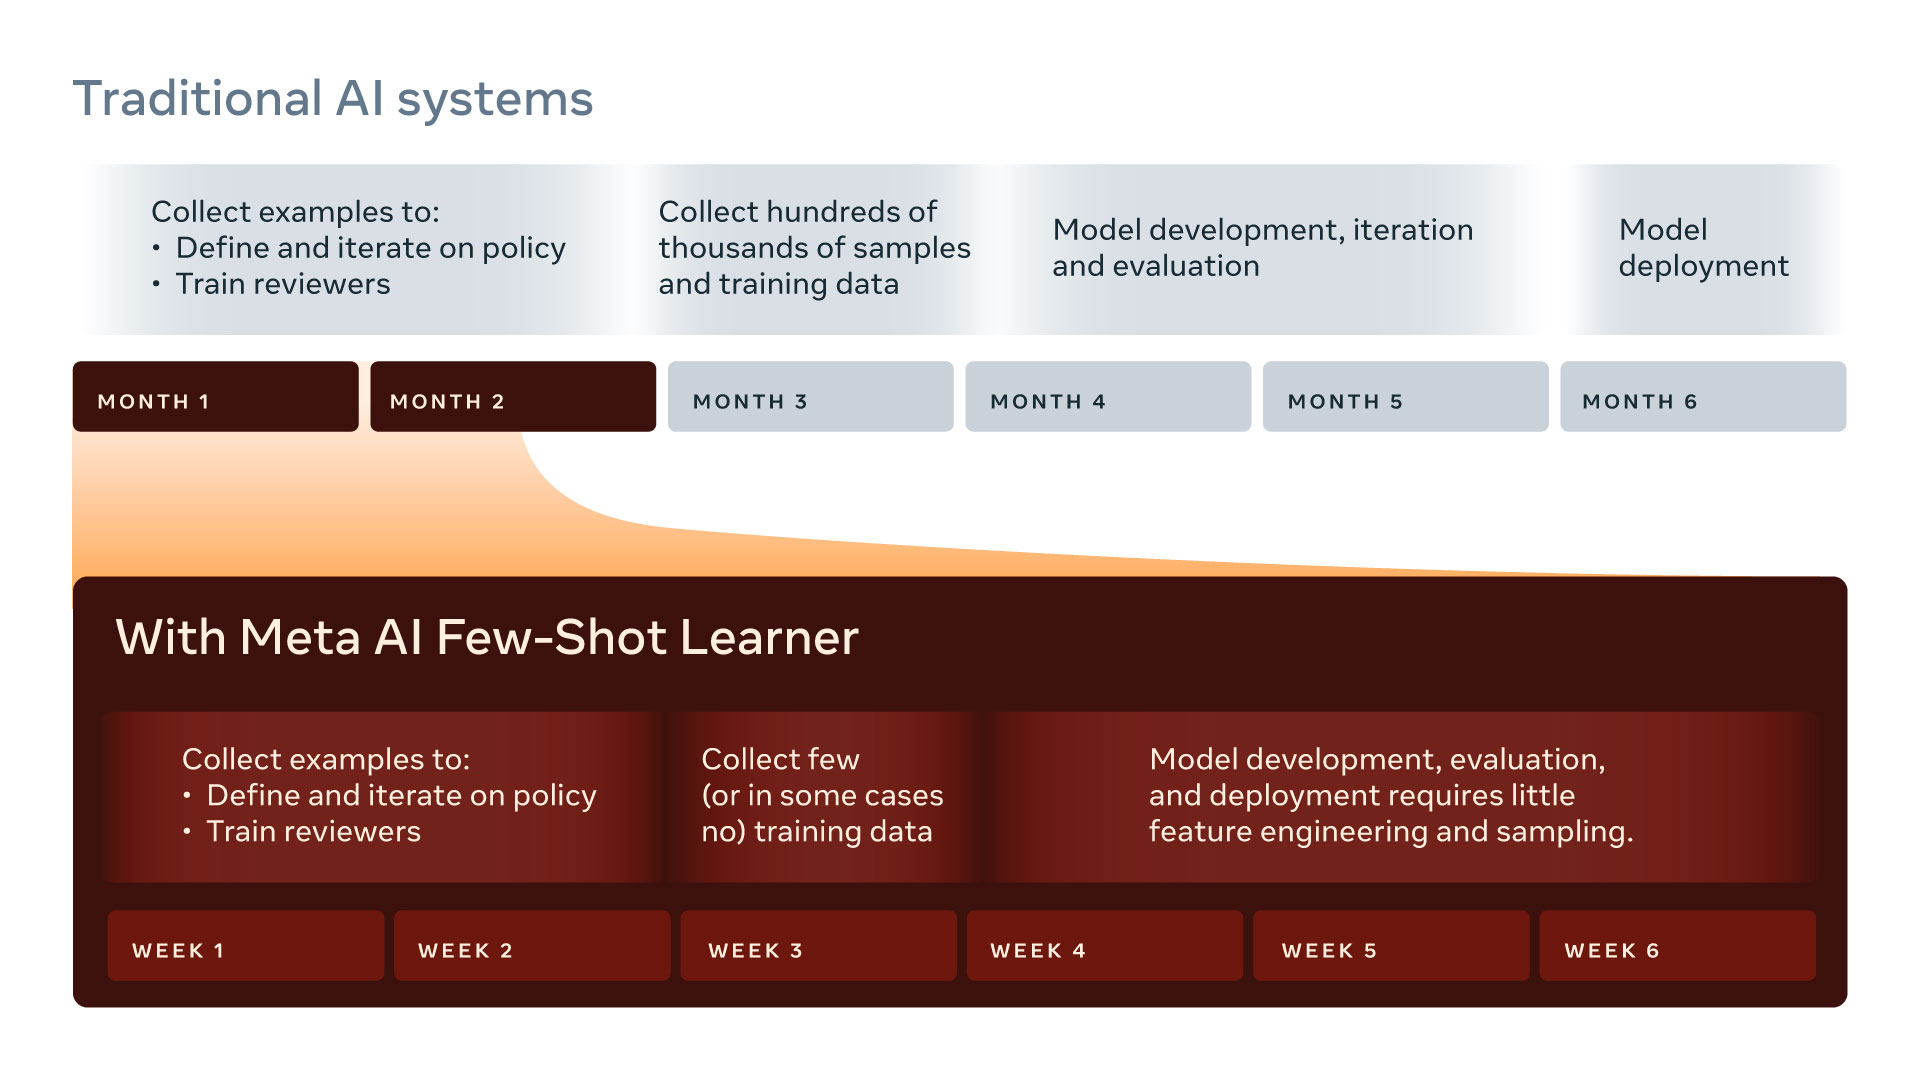
\includegraphics[width=.8\textwidth]{images/fsl_timeline}
    \caption{source: \cite{site:AIart2}}
  \end{figure}
\end{frame}

\begin{frame}{Today's technology}
  \begin{figure}
    \centering
    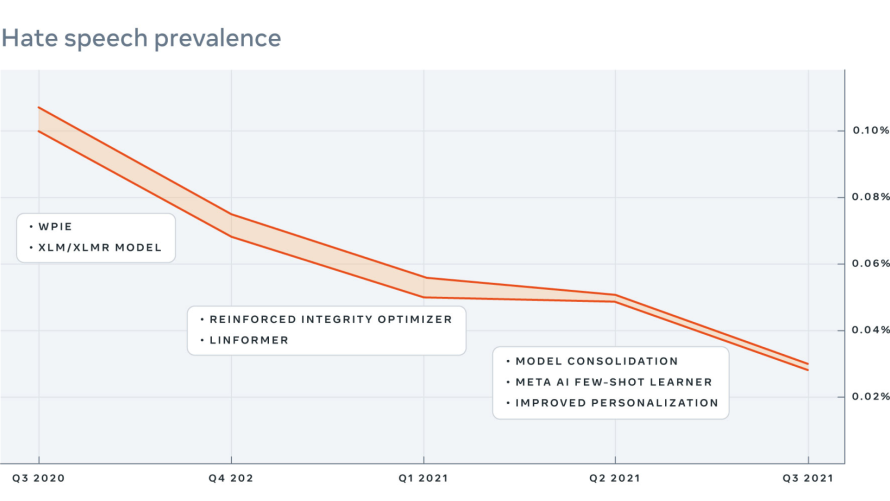
\includegraphics[width=.8\textwidth]{images/fsl_chart}
    \caption{source: \cite{site:AIart}}
  \end{figure}
\end{frame}

\begin{frame}
  \begin{enumerate}
  \item What kind of innovation is this?
  \item How does this innovation affect Meta business model?
  \end{enumerate}
\end{frame}

\section{New value in the business model}
\begin{frame}{Business model innovation}
  \begin{figure}
    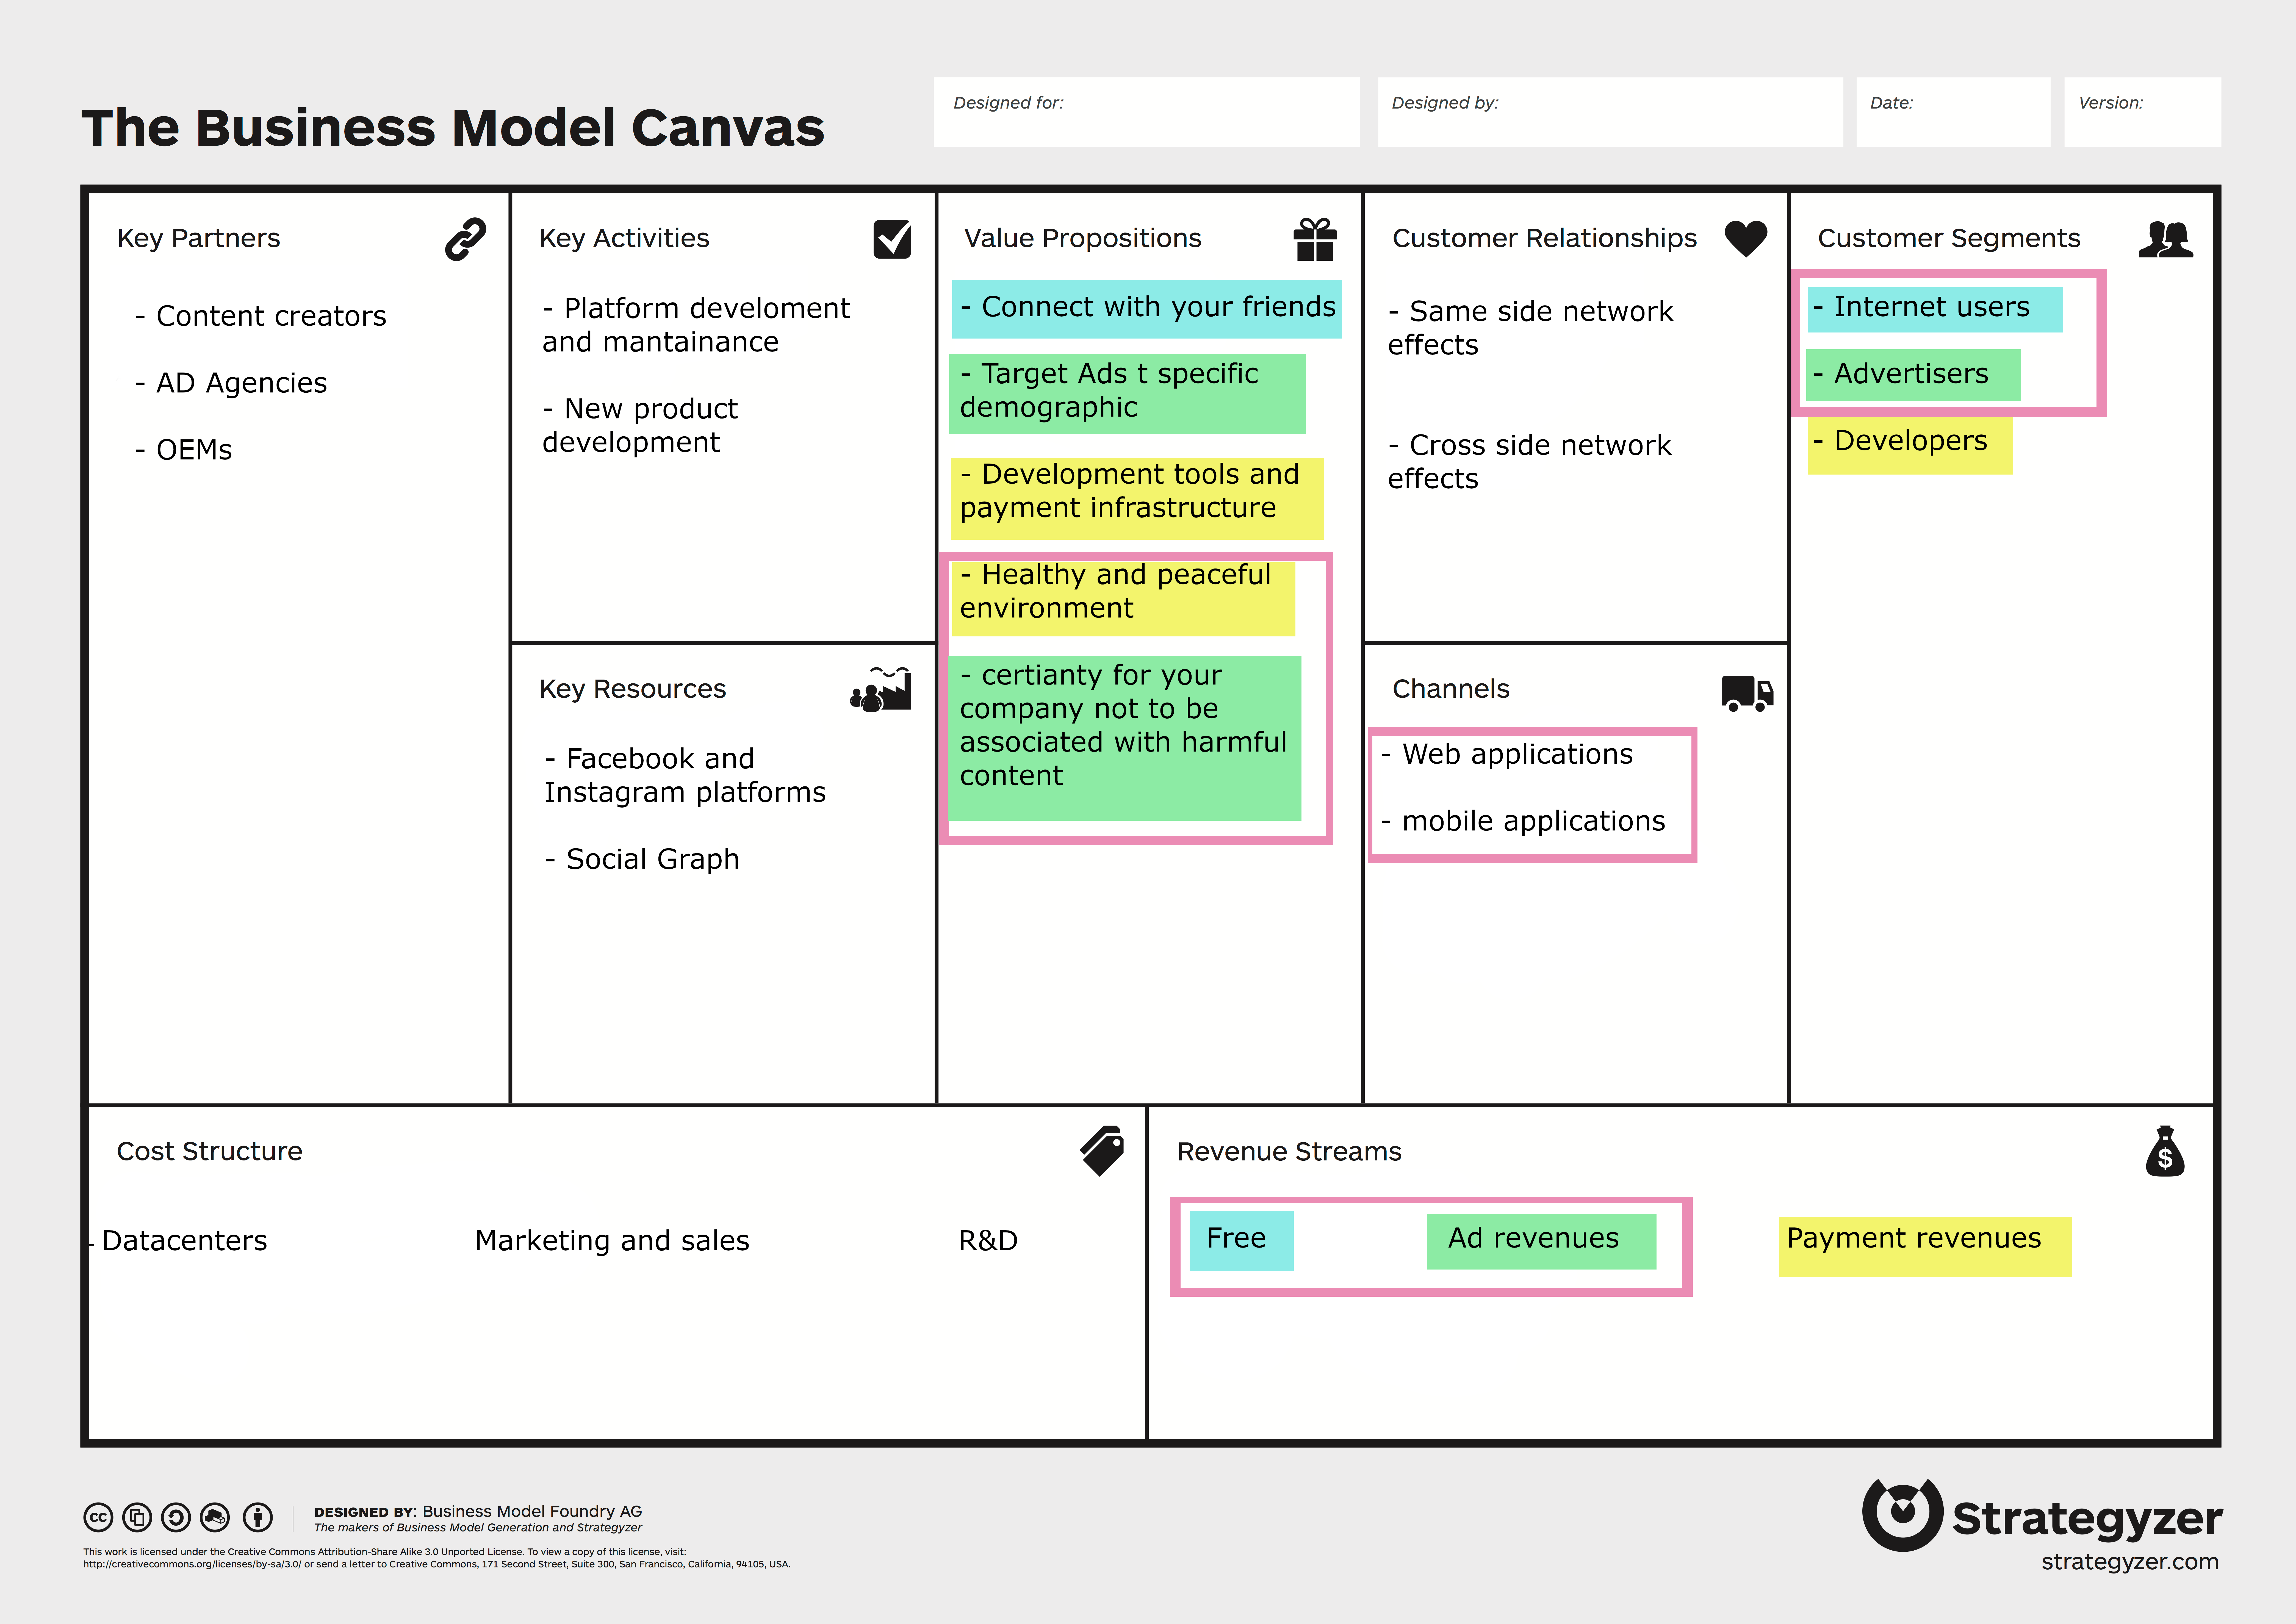
\includegraphics[width=\textwidth]{images/newcanvas.png}
  \end{figure}
\end{frame}

\section*{This is}
\begin{frame}{The end}
\centering Thank you!
\end{frame}

\section*{References}
\begin{frame}{References}
  \printbibliography
\end{frame}

\end{document}